\documentclass[runningheads,a4paper]{llncs}

\usepackage{amssymb}
\usepackage{amsmath}
\setcounter{tocdepth}{3}
\usepackage{graphicx}
%EW:
%\usepackage{subcaption}
\usepackage{caption}
\usepackage{float}
\usepackage[caption = false]{subfig}
\usepackage{multirow}
\usepackage[outdir=../eps]{epstopdf}
%:EW
\usepackage{algorithm}
\usepackage{algorithmic}
\usepackage{psfrag}
\usepackage{url}

%EW:
\captionsetup[table]{skip=10pt}
\graphicspath{{../eps/}}
\DeclareGraphicsExtensions{.eps}
%:EW

\urldef{\mailsa}\path|jarabas@elka.pw.edu.pl|
\urldef{\mailsb}\path|ewarchul@mion.elka.pw.edu.pl|
\newcommand{\keywords}[1]{\par\addvspace\baselineskip
\noindent\keywordname\enspace\ignorespaces#1}

\newcommand{\wek}[1]{
    {\bf #1} 
}
\newcommand{\mat}[1]{
    {\bf #1} 
}
\newcommand{\srednia}[1]{
    \langle #1 \rangle 
}

\newcommand{\argmax}{\operatornamewithlimits{argmax}} 

\newcommand{\FES}{
    \text {FES} 
}

\newcommand{\MAXFES}{
    \text{MAXFES} 
}

\newcommand{\ffrac}[2]{\ensuremath{\frac{\displaystyle #1}{\displaystyle #2}}}

\begin{document}

\mainmatter  
\title{Investigation of step-size adaptation methods for CMA-ES based on population midpoint fitness}

\titlerunning{Step-size adaptation for CMA-ES based on population midpoint fitness}

\author{Jaros\l aw Arabas\and Eryk Warchulski}
%
\authorrunning{J.Arabas \and E.Warchulski}
\institute{Warsaw University of Technology, Institute of Computer Science, Poland\\ 
\mailsa, \mailsb 
}

%\toctitle{Investigation of step-size adaptation methods for CMA-ES based on population midpoint fitness}
%\tocauthor{Jaros\l aw Arabas\and Eryk Warchulski}


\maketitle


\begin{abstract}

In this paper, we introduce and investigate three different new methods to control step size multiplier for the Covariance Matrix Adaptation Evolution Strategy (CMA-ES). The methods are intended to substitute the Cumulative Step Adaptation rule (CSA) that is a standard method to control step-size in CMA-ES. All investigated methods are based on the comparison of fitness values between the population midpoint and the offspring. All methods reveal linear convergence for the quadratic fitness function. 

In the first two methods, $\sigma$ is increased when the success ratio exceeds 1/5 and is decreased when the success ratio falls below 1/5. The success ratio in each iteration is defined as a fraction of the number of points generated in that iteration whose fitness value exceeds the fitness of the weighted mean (for the first method) or the simple arithmetic mean (for the second method) of points from the previous iteration.  In the third approach, $\sigma$ is increased when the fitness of the current iteration midpoint is located below a certain percentile of the fitness values in that population.

According to the results of tests with the use of  CEC'2013 and CEC'2017 benchmark sets, two introduced methods based on the population midpoint fitness analysis yielded very good results. The computational overhead was significantly smaller than in the case of CSA.

\end{abstract}
\keywords{CMA-ES, 1/5 success rate rule, CSA}
\section{Introduction}


Covariance Matrix Adaptation Evolution Strategy (CMA-ES) \cite{HansenOstermeier01} has been among the leading methods in black-box global optimization competitions. In each iteration, the method generates a population of random points using a multivariate normal distribution whose parameters --- the expectation vector and the covariance matrix --- are maintained by the method. In each iteration, the parameters are modified by analyzing the distribution of fitness values of generated points, according to the adaptation formula called CMA (Covariance Matrix Adaptation). In effect, the probability density function of the distribution to generate points tends to roughly approximate the fitness function shape in the area covered by the populations. 

Dynamics of the probability distribution adaptation by CMA is improved by introducing the third adaptive parameter --- the step-size multiplier --- that is used to multiply the random values generated using the aforementioned normal distribution. The canonical version of CMA-ES adapts the step-size multiplier by comparing the actual trajectory of the expectation vector with a hypothetical trajectory that would be observed when the fitness would be a constant function. This adaptation mechanism is called the Cumulative Step Adaptation (CSA).

CMA-ES has proved efficient in global optimization in real-space. It has been the basic algorithm for a family of methods that won black-box optimization competitions that have been regularly organized at evolutionary computation conferences like GECCO or CEC. Yet the very impressive effectiveness of CMA-ES is occupied by a considerable computational effort that is needed to perform matrix operations. Therefore researchers present various simplifications of CMA-ES, usually at the expense of the algorithm efficiency. Researchers often change the CMA procedure, usually by reducing the accuracy of the matrix update. Some representative papers on that issue are \cite{Poland2001,Loshchilov2017,SMAES}. Much fewer papers are devoted to the CSA rule.   

In this paper, we focus on the procedure to control the step-size. The research was motivated by the results reported in \cite{Arabas17,Biedrzycki17}. It was shown there that the efficiency of CMA-ES could be improved by computing fitness of the population midpoint. Here we demonstrate that the information about midpoint fitness can facilitate the step-size adaptation rule. We introduce and examine three example methods to control the step-size that use the information about midpoint fitness. 

The first method takes into account the expectation vector of the distribution used to generate points. If its fitness is smaller than 20\% of generated points then the steps-size is decreased, otherwise, it is increased. The second method works similarly, but, instead of the expectation vector, it uses the arithmetic mean of all points generated in the previous iteration. The third method looks at the arithmetic mean of points from the current iteration. It increases or decreases the step-size multiplier value when the fitness of the current population mean is smaller or greater than a certain fraction of the current population.

The paper is composed as follows. Section 1 briefly introduces the research problem. In Section 2, we outline the considered version of CMA-ES. We discuss the standard CSA rule to control the value of the step-size multiplier. We present two alternative rules of step-size control taken from the literature. Section 3 introduces three methods to control the step-size which are based on a comparison of fitness values of points generated by CMA-ES and their midpoint. Section 4 presents the results of simulations that were obtained by CMA-ES coupled with various methods to control step-size, for linear and quadratic fitness functions. We discuss the convergence rate for the compared methods as well as the computational overhead that is introduced by the use of step-size control procedures.  In Section 5 we present the results of testing CMA-ES, which was coupled with different step-size control rules. We use two benchmark sets that were introduced for CEC'2013 and CEC'2017 black-box optimization competition. Section 6 concludes the paper. 


\section{Step-size adaptation methods for CMA-ES}

Algorithm 1 presents an outline of the considered version of CMA-ES. The method maintains three parameters: the expectation vector $\wek{m}^t$, the covariance matrix $\mat{C}^t$ and the step-size multiplier $\sigma^t$, which are the parameters of the multinomial normal distribution used to generate points; the upper index $t$ stands for the iteration number.
In each iteration the algorithm uses the multinomial normal distribution with zero expectation and the covariance matrix $\mat{C}^t$ to generate the set of vectors $\{\wek{d}_1^t,...,\wek{d}_\lambda^t\}$ (line 6).% The vectors are used to define points $\{\wek{x}_1^t,...,\wek{x}_\lambda^t\}$ whose fitness is evaluated (lines 7,8). 
Then the populations of vectors $\wek{d}_i^t$ is sorted according to their fitness values (line 9) such that it holds:
\begin{equation*}
q(\wek{m}^t+\sigma^t \wek{d}_i^t) \leq q(\wek{m}^t+\sigma^t \wek{d}_{i+1}^t)
\end{equation*}
where $q: {\mathbb R}^n \rightarrow R$ stands for the fitness function.
For brevity, we shall denote $\wek{x}^t_i=\wek{m}^t+\sigma^t \wek{d}_i^t$.

%\begin{algorithm}[h]
%\caption{CMA-ES}
%\label{alg-CMA-ES}
%\begin{algorithmic}[1]
%\STATE $t \gets 1$
%\STATE initialize$(\wek{m}^1,\sigma^1, C^1)$
%\STATE $\wek{p}_c^1 \gets \wek{0}$, $\wek{p}_\sigma^1 \gets \wek{0}$
%\WHILE{!stop}
   %\FOR{$i=1$ \TO $\lambda$}
      %\STATE $ \wek{d}_i^t \sim N(\wek{0}, \mat{C}^t) $
      %\STATE evaluate $(\wek{x}_i^t)$
   %\ENDFOR
   %\STATE sort $ \left(\{ \wek{x}_i^t \} \right) $
   %\STATE $\wek{\Delta}^{t} \gets \sum_{i=1}^\mu w_i \wek{d}_i^t $
   %\STATE $\wek{m}^{t+1} \gets \wek{m}^{t+1} + \sigma^t \Delta^t $
   %\STATE $\wek{p}_c^{t+1} \gets (1-c_p)\wek{p}_c^t + \sqrt{\mu c_p(2-c_p)} \cdot \Delta^t$
   %\STATE $\mat{C}^{t+1} \gets (1-c_1-c_\mu)\mat{C}^t + c_1 \mat{C}^t_1 + c_\mu  \mat{C}^t_\mu$ where \newline
%$\qquad \mat{C}_\mu^t=\frac{1}{\mu_\text{eff}}\sum_{i=1}^\mu w_i(\wek{d}_i^t)(\wek{d}_i^t)^T$, $\mu_\text{eff}=1/\left(\sum_{i=1}^\mu (w_i)^2\right)$ \newline
%$\qquad \mat{C}_1^t=(\wek{p}_c^t)(\wek{p}_c^t)^T$
   %\STATE $\sigma^{t+1} \gets $ CSA $(\sigma^t, \mat{C}^{t}, \Delta^t)$ 
   %\STATE $t \gets t+1$
%\ENDWHILE
%\end{algorithmic}
%\end{algorithm}

Out of $\lambda$ generated vectors, a subset of $\mu$ elements with the lowest fitness value is selected to perform an adaptation of the algorithm parameters.
The expectation vector $\wek{m}^t$ is modified by adding the weighted mean of selected vectors $\wek{\Delta}^t$ (lines 10,11). 

The covariance matrix $\mat{C}^t$ is updated by formula (line 13) that takes into account two summands. The first summand is a rank-$\mu$ matrix $\mat{C}^t_\mu$ which is a weighted sum of the outer products of $\mu$ selected vectors $\wek{d}_i^t$. The second summand is a rank-1 matrix $\mat{C}^t_1$ being the outer product of the vector $\wek{p}_c^t$. This vector accumulates values of $\wek{\Delta}^t$ from previous iterations (line 12).

The step-size multiplier $\sigma^t$ is updated using the Cumulative Step Adaptation rule which is discussed in more detail in the next subsection. 



\subsection{Cumulative Step-size Adaptation}

Consider the case when the fitness function is a constant function. Then the indices of vectors $\wek{d}_i^t$ have no correlation with their location in space. Consequently, since the selected vectors $\wek{d}_i^t$ are independent and normally distributed with zero mean and the covariance $\mat{C}^t$, the vectors $(\mat{C}^t)^{-1/2} \wek{d}_i^t$ are distributed with zero mean and the identity covariance matrix. Then the vector $(\mat{C}^t)^{-1/2} \wek{\Delta}^t$ will be distributed with zero mean and the covariance matrix equal to:
\begin{equation}
\Sigma((\mat{C}^t)^{-1/2} \wek{\Delta}^t) = \sum_{i=1}^\mu (w_i)^2 \mat{I}=\frac{1}{\mu_\text{eff}} \mat{I}
\label{eq:01}
\end{equation}
The vectors $(\mat{C}^t)^{-1/2} \wek{\Delta}^t$ will be also mutually independent. 

%\floatname{algorithm}{Procedure}
%\setcounter{algorithm}{0}
%\begin{algorithm}[h]
%\caption{CSA}
%\begin{algorithmic}[1]
   %\STATE $\wek{p}_\sigma^{t+1} \gets (1-c_s)\wek{p}_\sigma^t + \sqrt{\mu_\text{eff} c_s(2-c_s)} \cdot (\mat{C}^t)^{-\frac{1}{2}}\wek{\Delta}^t$
   %\STATE $\sigma^{t+1} \gets \sigma^t \exp\left(\frac{c_s}{d_\sigma} \left(\frac{\| \wek{p}_\sigma^{t+1} \|}{E\|N(\wek{0},\mat{I})\|}-1\right)\right) $

%\end{algorithmic}
%\end{algorithm}

The CSA method (see Procedure 1) takes advantage from this observation. Vectors $(\mat{C}^t)^{-1/2} \wek{\Delta}^t$ from consecutive iterations are accumulated into the vector  $\wek{p}_\sigma^{t}$. In the case of constant fitness function, the vector $\wek{p}_\sigma^{t}$ will behave in consecutive iteration as if it were randomly generated with zero mean and identity covariance, since its covariance matrix is
\begin{equation}
\Sigma(\wek{p}_\sigma^{t+1}) = (1-c_s)^2 \Sigma(\wek{p}_\sigma^{t}) + \mu_\text{eff} c_s(2-c_s) \Sigma((\mat{C}^t)^{-1/2} \wek{\Delta}^t)
\end{equation}
Taking into account \eqref{eq:01} and assuming that $\Sigma(\wek{p}_\sigma^{t})=\mat{I}$ we obtain:
\begin{equation}
\Sigma(\wek{p}_\sigma^{t+1}) = (1-c_s)^2 \mat{I} + \mu_\text{eff} c_s(2-c_s) \left(\frac{1}{\mu_\text{eff}}\mat{I}\right) = \mat{I}
\end{equation}
Hence, if the fitness function is a constant function then the vector $\wek{p}_\sigma^{t}$ can be treated as a random variable with zero mean and the identity covariance matrix. Then it will hold
$$ E\|\wek{p}_\sigma^{t}\| = E\|N(\wek{0},\mat{I})\| $$
and 
$$ E\|\sigma^{t+1}\| = E\|\sigma^{t}\| $$

For an arbitrary fitness function, the length of $(\mat{C}^t)^{-\frac{1}{2}}\wek{\Delta}^t$ will differ from the case of the constant fitness. Two factors will influence the change of $ E\|\wek{p}_\sigma^{t}\|$:
\begin{enumerate}
\item The average length of $(\mat{C}^t)^{-\frac{1}{2}}\wek{\Delta}^t$ is smaller when the selection process prefers shorter vectors $\wek{d}_i^t$, which typically takes place when the algorithm is nearby the local optimum. Then $\sigma^t$ will be reduced. Contrarily, if longer vectors are selected, then this may indicate a saddle and will result in increasing $\sigma^t$.
\item If the consecutive vectors $\wek{\Delta}^t$ are positively correlated then the length of 
$\wek{p}_\sigma^{t}$ will increase along with the iteration number. Such a situation may appear when the populations are located on a slope towards optimum. In effect of increasing length of $\wek{p}_\sigma^{t}$ the step-size will increase. Due to the same mechanism, a negative correlation of consecutive vectors $\wek{\Delta}^t$ will result in decreasing $\sigma^t$.
\end{enumerate}

\subsection{Step-size control inspired by the one-fifth success rule}

The one-fifth success rule \cite{Schwefel95} is a method to control the step-size that was originally applied for the (1+1)-ES algorithm. It has been verified that the optimization progress of (1+1)-ES is highest when the ratio of successful mutation is kept around 1/5. Therefore, a record of successful mutation should be kept for (1+1)-ES. If the ratio of successful mutations falls below 1/5 then the step-size should decrease, and if it exceeds 1/5 then the step size should be reduced.


The method inspired by the one-fifth rule was defined to control the step-size for (1+1)-CMA-ES \cite{Suttorp09}. This algorithm maintains a single point $\wek{m}^t$, a covariance matrix $\mat{C}^t$, and a step size multiplier $\sigma^t$. In each iteration one vector $\wek{d}^t$ is generated from the multinomial normal distribution with covariance matrix $\mat{C}^t$. An offspring point is defined as $\wek{x}^t=\wek{m}^t+\sigma^t\wek{d}^t$. If the fitness value of $\wek{x}^t$ is smaller than $\wek{m}^t$, the offspring supersedes its parent, and the covariance matrix $\mat{C}^t$ is made in a fashion similar to CMA-ES. The step-size adaptation is defined in a way inspired by the one-fifth rule --- see Procedure 2.

%\begin{algorithm}[h]
%\caption{One-fifth rule for (1+1)-CMA-ES}
%\begin{algorithmic}[1]
   %\IF {$q(\wek{x}^t)<q(\wek{m}^t)$}
   %\STATE $p_s^{t+1} \gets (1-c_s) p_s^t + c_s $
   %\ELSE
   %\STATE $p_s^{t+1} \gets (1-c_s) p_s^t $
   %\ENDIF
   %\STATE $\sigma^{t+1} \gets \sigma^t \exp\left(\frac{1}{d} \cdot \frac{p_s-p_\text{target}}{1 - p_\text{target}}\right) $ 
%\end{algorithmic}
%\end{algorithm}

The value $p_\text{succ}^{t}$ accumulates the ratio of succesful mutations. The smoothing factor $c_p$, the damping factor $d$ and the target success rate $p_\text{target}$ are set by the user. The settings suggested in \cite{Suttorp09} are $c_p=1/12, d=1+n/2, p_\text{target}=2/11$. 

The CSA rule adapts the value of $\sigma^t$ in CMA-ES by looking on distribution of $\lambda$ points generated in each iteration, while the one-fifth rule needs a number that estimates the success rate. The Median Success Rule (MSR), which was introduced in \cite{Elhara13}, looks at percentiles of fitness values observed in points generated in consecutive iterations. 

%\begin{algorithm}[h]
%\caption{Median Success Rule}
%\begin{algorithmic}[1]
   %\STATE $K_\text{succ} = \left|\{i: q(\wek{x}_i^t) < q(\wek{x}_{k\cdot\lambda}^{t-1})\}\right|/\lambda$
   %\STATE $z^t \gets (\frac{2}{\lambda} \cdot \left(K_\text{succ}-\frac{\lambda+1}{2}\right)$
   %\STATE $p_s^{t+1} \gets (1-c_s)p_s^t + c_s \cdot z^t$
   %\STATE $\sigma^{t+1} \gets \sigma^t \exp\left(\frac{p_s}{d} \right) $

%\end{algorithmic}
%\end{algorithm}


With $P_i(X)$ denote the $i$-th percentile of values conatined in the set $X$. In the MSR method, the median fitness of the current population $P_{0.5}(\{q(\wek{x}^t_i)\})$ is compared with a certain fitness percentile $P_{k}(\{q(\wek{x}^{t-1}_i)\})$ from the previous population. It is argued in \cite{Elhara13} that a desired situation is when it holds
\begin{equation}
Prob\{P_{0.5}(\{q(\wek{x}^t_i)\}) < P_{k}(\{q(\wek{x}^{t-1}_i)\})\} \approx 1/2
\end{equation}       
Hence, the desired success ratio is expected to be around one-half instead of one-fifth. According to the results of experiments provided in \cite{Elhara13}, the following settings are advisable: $k=0.3, c_s=0.3, d=2(n-1)/n$.

\section{Step-size adaptation based on the midpoint fitness}

Generalization of the one-fifth rule to work for the algorithm that generates $\lambda>1$ points, such as CMA-ES, is neither straightforward nor unique. Here we suggest three possible generalizations. All of them need to evaluate the fitness of a population midpoint. This causes some additional effort in terms of the number of fitness evaluations, which might be a drawback when a limited budget of the number of fitness evaluations is assumed. However, as it was shown in \cite{Arabas17}, computing of the population midpoint may improve a precise location of local optima and may serve as a basis to improve the overall efficiency of CMA-ES \cite{Biedrzycki17}. Therefore, we present three methods that take into account the values of fitness of population midpoints.


The first method, which is outlined in Procedure 4, is inspired by the one-fifth rule for (1+1)-CMA-ES. It looks at $\overline{\wek{x}}^{t-1}$ --- the midpoint of points from the previous iteration. The success ratio $p_s$ is defined as the number of points from the current iteration whose fitness is smaller than the previous iteration midpoint. The method does not use any smoothing procedure for $p_s$. Suggested values of parameters are $ p_\text{target}=1/5, d=3$. 
%
%\begin{algorithm}[h]
%\caption{Previous Population Midpoint Fitness (PPMF) rule}
%\begin{algorithmic}[1]
   %\STATE $\overline{\wek{x}}^{t-1}=\frac{1}{\lambda}\sum_{i=1}^\lambda \wek{x}_i^{t-1}$
   %\STATE evaluate $(\overline{\wek{x}}^{t-1})$
   %\STATE $p_s = \left|\{i: q(\wek{x}_i^t) < q(\overline{\wek{x}}^{t-1})\}\right|/\lambda$
   %\STATE $\sigma^{t+1} \gets \sigma^t \exp\left(\frac{1}{d} \cdot \frac{p_s-p_\text{target}}{1-p_\text{target}}\right) $

%\end{algorithmic}
%\end{algorithm}

The second method is outlined in Procedure 5. It is another attempt to directly apply the philosophy of the one-fifth rule. In (1+1)-ES, one parent generates one offspring by adding a normally distributed difference vector. In CMA-ES, normally distributed difference vectors $\wek{d}_i^t$ are used to generate new points around the point $\wek{m}^t$. Therefore, the point $\wek{m}^t$ acts as a parent, and its fitness value should be taken for comparison with all newly generated points. Suggested values of parameters are $ p_\text{target}=1/5, d=8$. 
% 
%\begin{algorithm}[h]
%\caption{Current Population Expectation Fitness (CPEF) rule}
%\begin{algorithmic}[1]
   %\STATE evaluate $(\wek{m}^t)$
   %\STATE $p_s = \left|\{i: q(\wek{x}_i^t) < q(\wek{m}^t)\}\right|/\lambda$
   %\STATE $\sigma^{t+1} \gets \sigma^t \exp\left(\frac{1}{d} \cdot \frac{p_s-p_\text{target}}{1-p_\text{target}}\right)  $

%\end{algorithmic}
%\end{algorithm}

In contrast to the aforementioned methods based on the midpoint from the previous iteration, the third considered method looks at the current iteration. Note however that the current population midpoint $\overline{\wek{x}}^t$ is an estimator of $\wek{m}^t$ since the average of independent samples of a random variable estimates its mean. The method outline is presented in Procedure 6.
If the fitness of $\overline{\wek{x}}^t$ is better than the best point of $\wek{x}^t_i$  then the population has probably approached to the vicinity of a local optimum. Then the precision can be improved by reducing $\sigma^t$. Contrarily, if the population is located on a slope and the fitness function can be locally approximated as a linear function, then the population mean fitness $q(\overline{\wek{x}}^t)$ will be roughly equal the median fitness value of the population. 

In the considered method we compare  $q(\overline{\wek{x}}^t)$ with the $k$ percentile of the population fitness. In further text we report the results obtained for $k=0.09$, and the step-size multiplier was set to $\alpha=0.83$, according to \cite{Schwefel95}.

%\begin{algorithm}[h]
%\caption{Current Population Midpoint Fitness (CPMF) rule}
%\begin{algorithmic}[1]
   %\STATE $\overline{\wek{x}}^t=\frac{1}{\lambda}\sum_{i=1}^\lambda \wek{x}_i^t$
   %\STATE evaluate $(\overline{\wek{x}}^t)$
   %\STATE $p_s = \left|\{i: q(\wek{x}_i^t) < q(\overline{\wek{x}}^t)\}\right|/\lambda$
   %\IF {$p_s < k$}
   %\STATE $\sigma^{t+1} \gets \alpha \cdot \sigma^t $
   %\ELSE 
   %\STATE $\sigma^{t+1} \gets \alpha^{-1} \cdot \sigma^t $
   %\ENDIF

%\end{algorithmic}
%\end{algorithm}


\section{Convergence of CMA-ES with various step-size adaptations}
\subsection{Compared methods}

In this section we investigated rates of convergence and computing overhead of proposed methods. 
As mentioned in previous sections we considered five methods using different $\sigma$ adaptation rules:
  \begin{enumerate}
    \item CMA-ES-CSA
    \item CMA-ES-MSR
    \item CMA-ES-EXPTH
    \item CMA-ES-JA
    \item CMA-ES-QUANT
  \end{enumerate}

Each method used default settings for basic parameters suggested by authors execpt for 
population size $\lambda$. All methods generated $\lambda = 4N$ points in each iteration.
For CMA-ES-MSR to count $K_{succ}$ of better points in current population than $j$-th best point 
of the previous population we set $j$ as:

\begin{equation*}
j = 0.3\lambda.
\end{equation*}

\subsection{Fitness functions: linear, quadratic, gutter}

To illustrate and compare rates of convergence we used three different fitness landscapes i.e. linear (\ref{eq:1}), quadratic
(\ref{eq:2}) and gutter function (\ref{eq:3}).

\begin{align}
  f_{l}(\wek{x}) &= x_{1}  \label{eq:1} \\
  f_{q}(\wek{x}) &= \sum^{D}_{i = 1} x^{2}_{i} \label{eq:2} \\
  f_{g}(\wek{x}) &= x_{1} + \sum^{D}_{i = 2} x^{2}_{i}, \; \wek{x} \in \mathbb{R}^{D}  \label{eq:3}
\end{align}

To assess the rates of convergence, each function was treated in a minimalization manner and we recorded the fitness of the 
arthimetic mean and the best point in the population. \\
The curves depicted in the figures below for iteration $t$ show the fitness of the best point and midpoint in the $t$th generation. \\ 
For each problem and algorithm, the mean point of population is initialized as:
\begin{equation*}
  \wek{m}_{i} = [100, \dots, 100]^{D}.
\end{equation*}

\subsection{Conclusions: convergence rate, benefits from using midpoint, search space dimension}
Results of simulations reveal that performance of non-CSA variants is competitive with CSA and MSR on both functions.
For n = 30 one can see that PPMF and CPEF have the biggest convergence rate among all considered methods.
Behavior of CPEF seems to be ambiguous due to significantly different rate of convergence depending on dimensionality — it may suggest potential inapplicability to problems with higher number of dimensions.
On the other hand, constant convergence rate of PPMF and outperforming behavior on sphere function regardless of dimensionality  encourage to formulate two contrary hypothesis: such improvement will be observed further or PPMF variant will be affected by premature convergence.
Possibility of such improvement or deterioration is verified in section \ref{section-5}


\begin{figure}[H]
\centering
  \subfloat[$f_q$, $D = 30$]{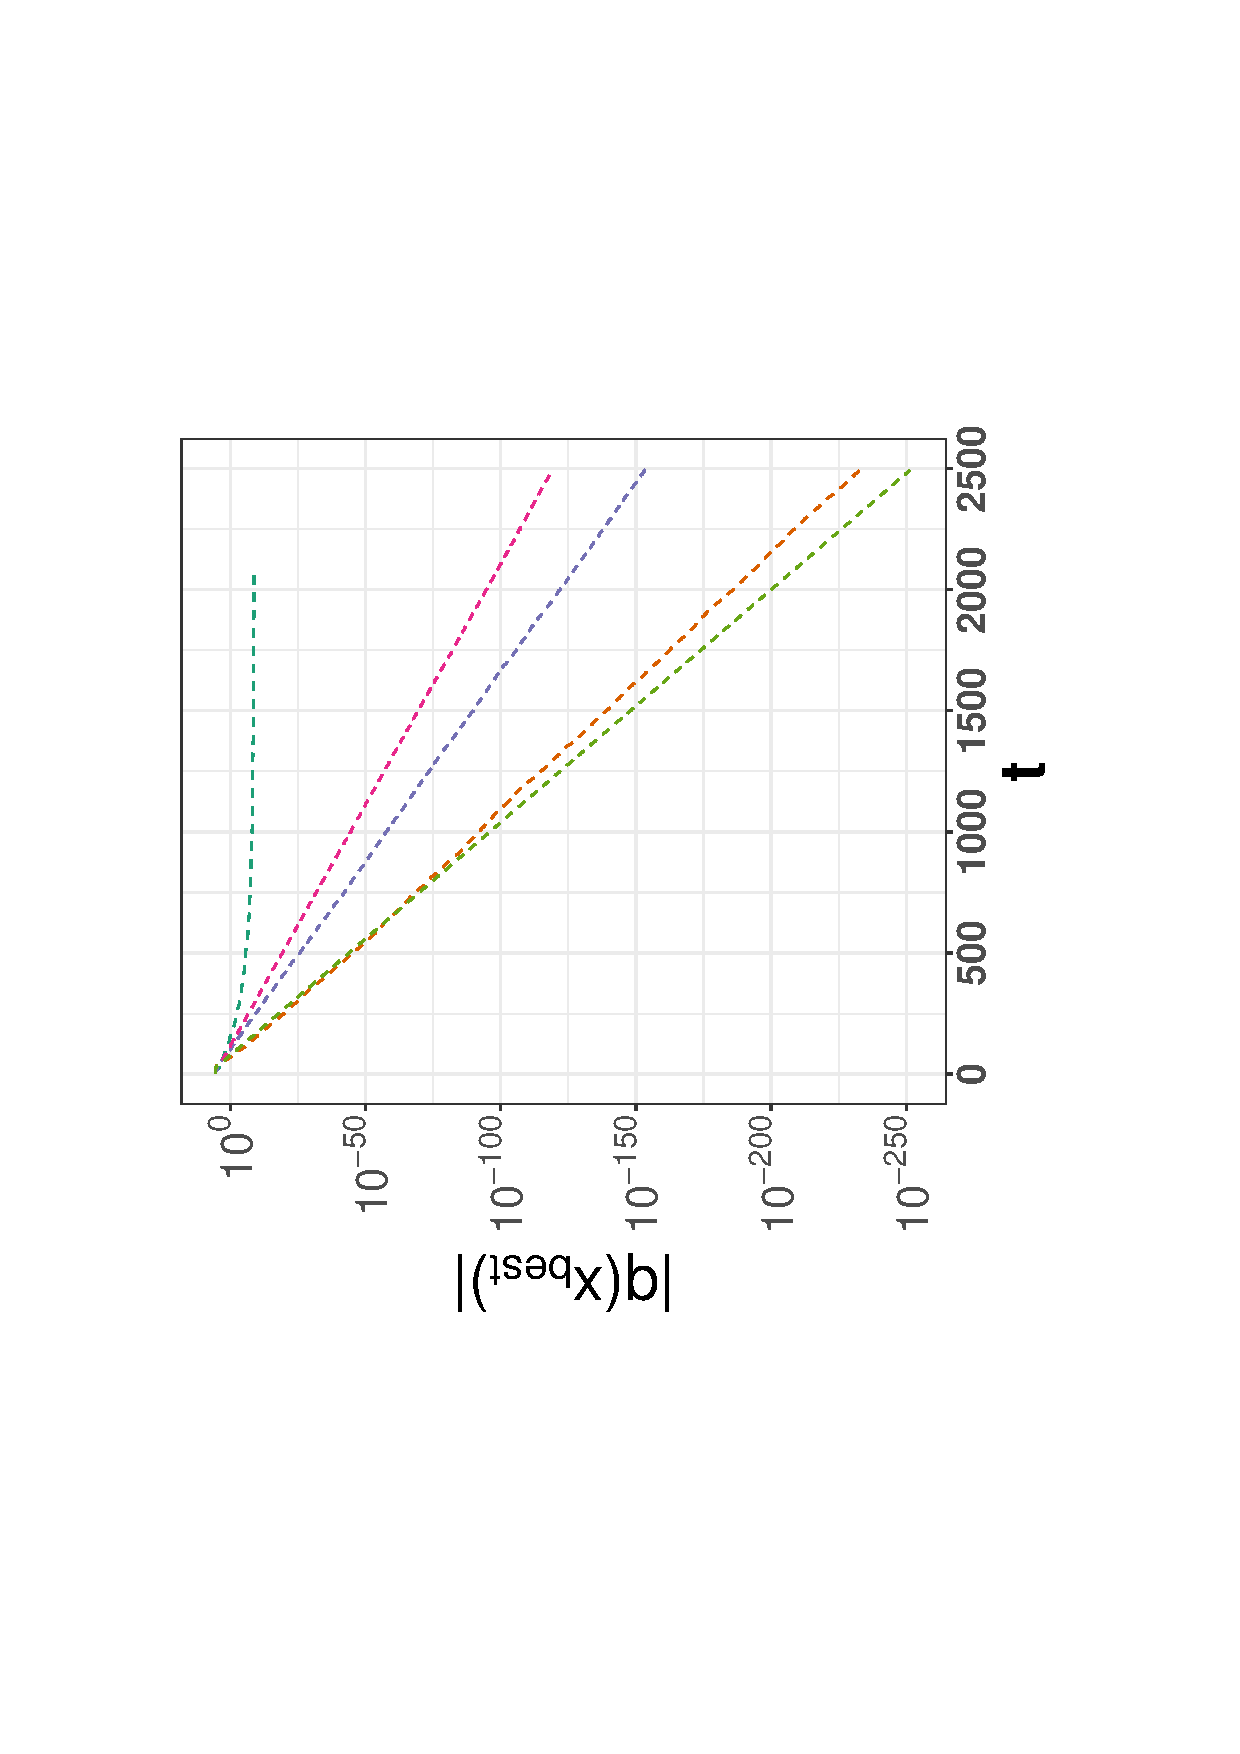
\includegraphics[width = 0.35\textwidth, angle = 270]{grid-sphere30}} 
  \subfloat[$f_q$, $D = 100$]{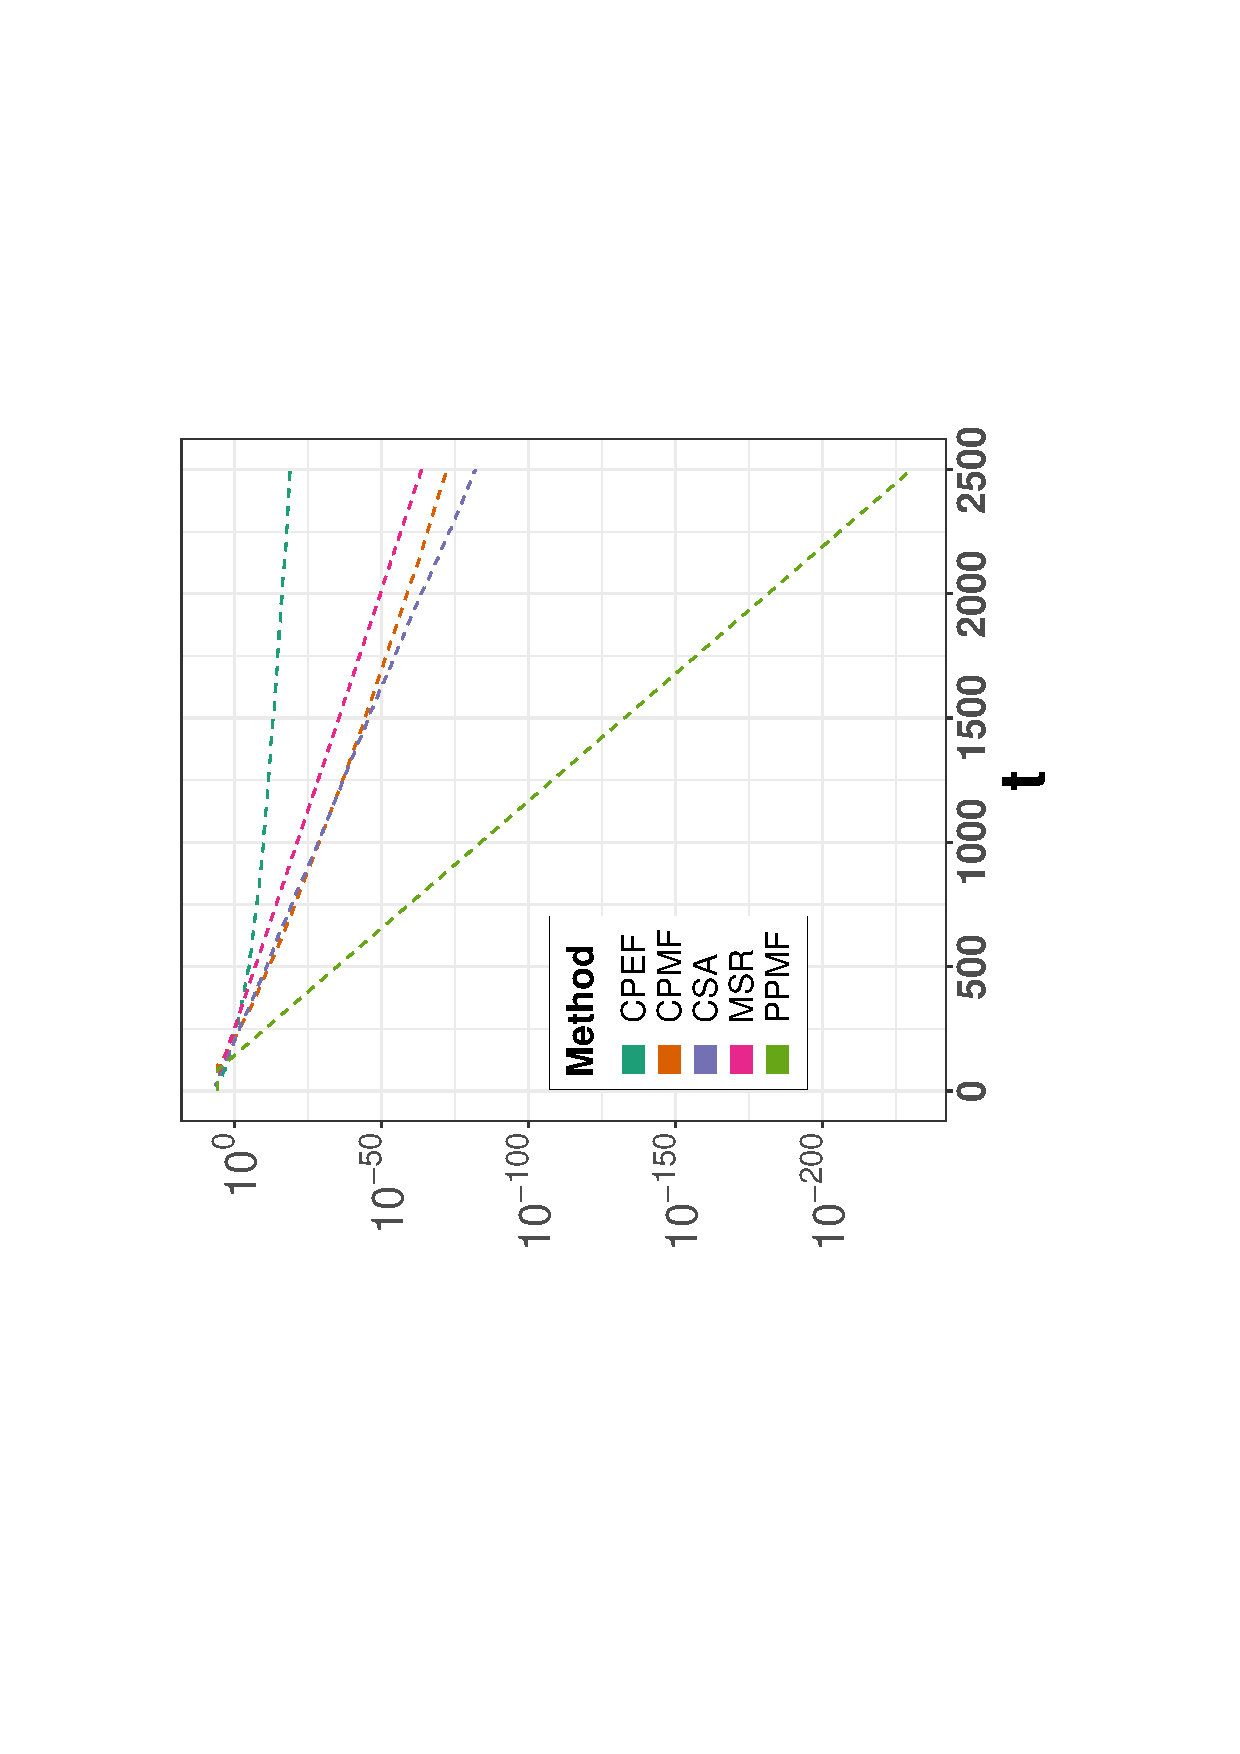
\includegraphics[width = 0.35\textwidth, angle = 270]{grid-sphere100}} \\
\subfloat[$f_l$, $D = 30$]{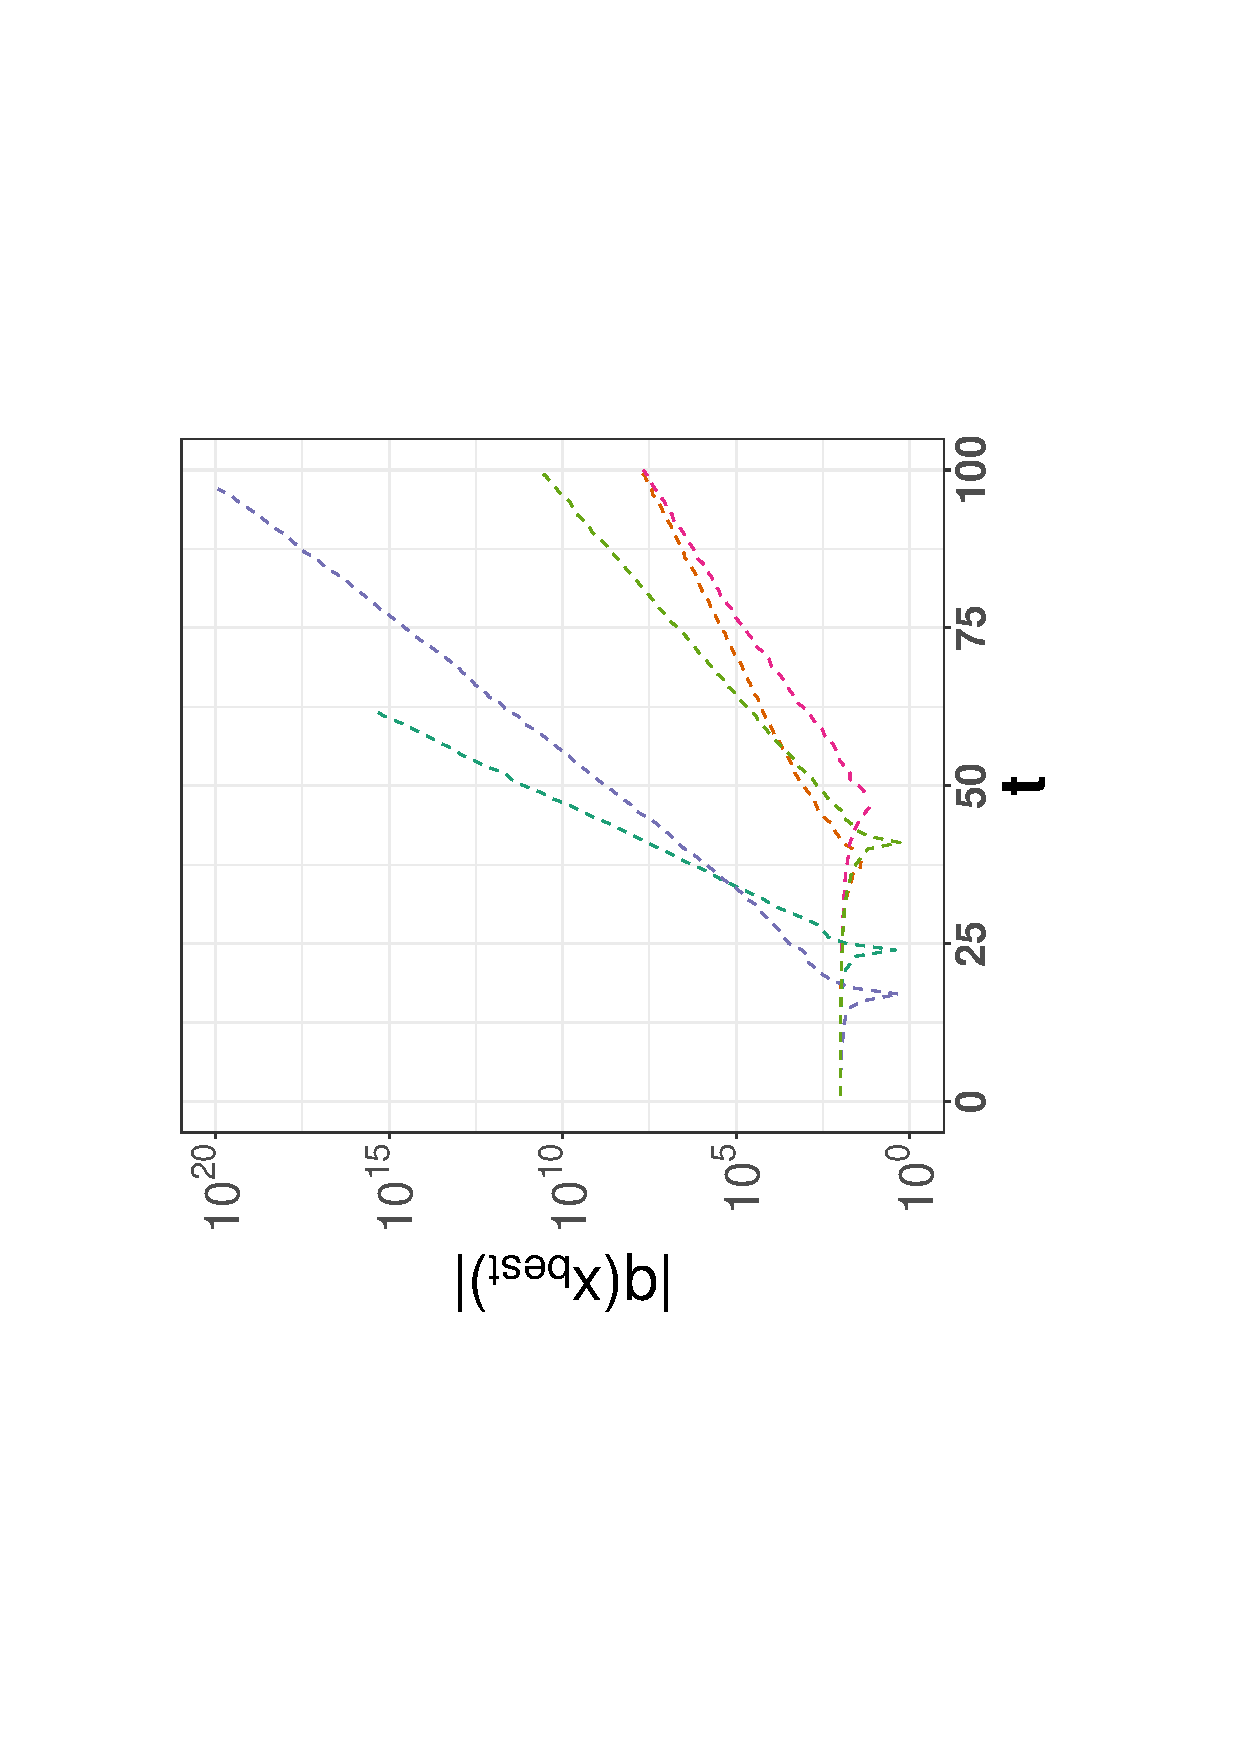
\includegraphics[width = 0.35\textwidth, angle = 270]{grid-linear30}} 
\subfloat[$f_l$, $D = 100$]{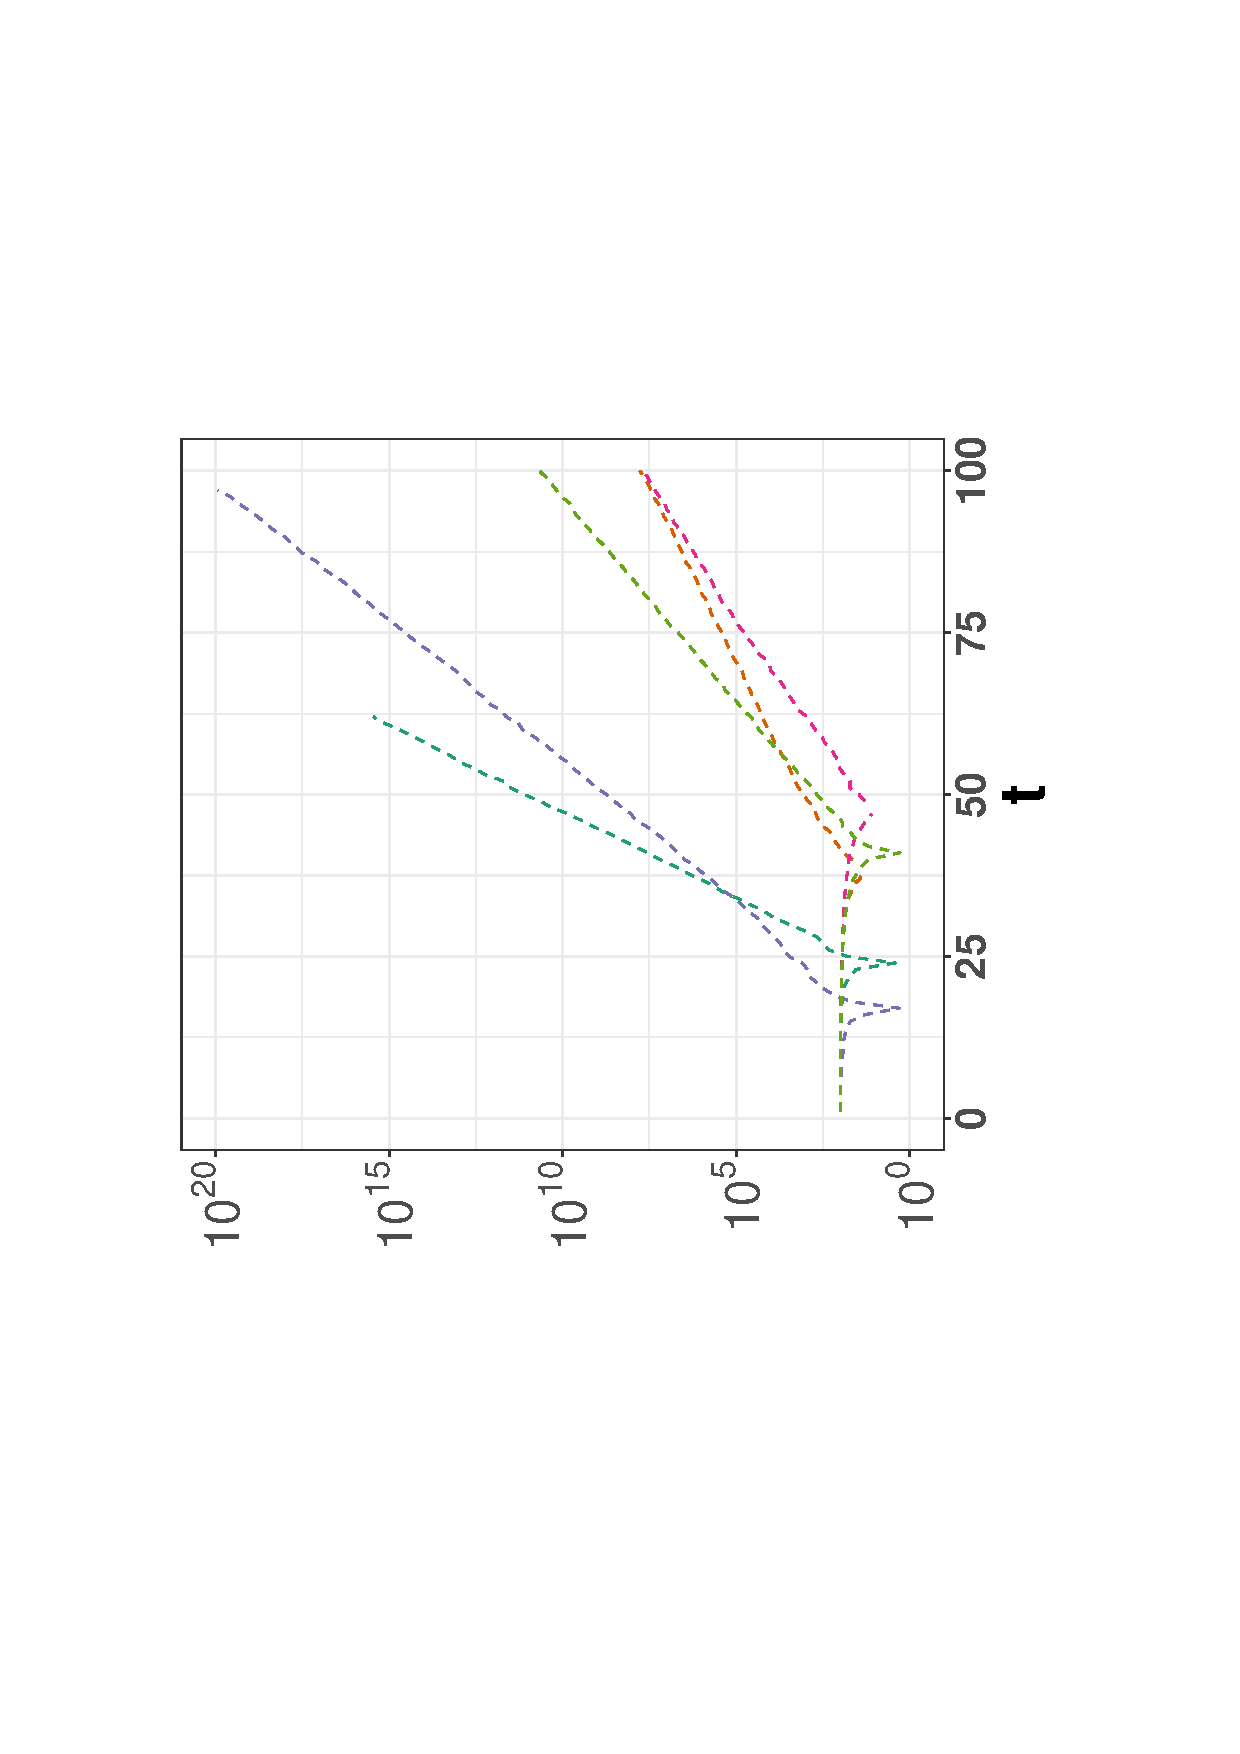
\includegraphics[width = 0.35\textwidth, angle = 270]{grid-linear100}} 
\caption{Convergence curves for different fitness landscapes.}
\label{some example}
\end{figure}

\section{Benchmarking step-size adaptation methods on CEC'2013 and CEC'2017}
\subsection{Overview of CEC'2013 and CEC'2017}

We tested the performance of proposed methods using standardized sets of single objective optimization problems i.e. CEC2017 \cite{cec2017} and CEC2013 \cite{2013}. Both of them are based on the benchmark set created in 2005 \cite{cec2005}.

Each problem in set is defined as follows:

\begin{equation*}
  \min_{\wek{x} \in [-100, 100]^{D}}\; f(\wek{x})
\end{equation*}

and should be considered as a black-box problem. One knows only dimensionality $D$, evaluation budget and value of global optimum. Note that the number of benchmark functions and functions by itself in CEC2013 and CEC2017 vary. 

CEC2013 has 28 functions which are dived into three groups: unimodal, multimodal and composition functions.
Structure of CEC2017 is similar with but with the addition of hybrid as a fourth group of function. 
Hybrid and composition functions are composed of several multimodal functions which are defined in such a way that in various regions of the
domain the dynamics of the objective function is dominated by different components of that composition.
Thus, the optimization algorithm must be able to capture these regularities over the whole run.
Structures of benchmarks are presented in the table below (\ref{cec-table}).

\begin{table}[H]
\label{cec-table}
\centering
\begin{tabular}{|c|c|c|l|l|l|c|c|}
\hline
Benchmark & Unimodal          & \multicolumn{4}{c|}{Multimodal}             & Hybrid                  & Composition             \\ \hline
CEC2017     & $f_1, \dots, f_3$ & \multicolumn{4}{c|}{$f_4, \dots, f_{10}$}   & $f_{11}, \dots, f_{20}$ & $f_{21}, \dots, f_{30}$ \\ \hline
CEC2013     & $f_1, \dots, f_5$ & \multicolumn{4}{c|}{$f_{6}, \dots, f_{20}$} &                         & $f_{21}, \dots, f_{28}$ \\ \hline
\end{tabular}
\caption{Structure of used benchmarks.}
\end{table}

We evaluated each algorithm with default settings for CEC benchmarks i.e. 51 independent repetitions for function, $10^{4}\cdot D$ objective function evaluations and dimensionality $D = 10, 30, 50$.

\subsection{Presentation of results using ECDF curves}

Instead of using tabular form of results presentation suggested by authors of CEC competitions, we decided to use ECDF (empirical cumulative distribution function) curve.
ECDF curve was proposed by Hansen \cite{Hansen-ecdf} as a convenient form of results aggregation. A single curve defines the average dynamics of the algorithm.
\\
More formally, let us suppose that one of the tested algorithms in $k$-th repetition of $D$-dimensional benchmark function $f \in \mathcal{F}$ recorded in generation $t$ value $Q^{f}_{k, D, t}$ 
which is the difference between the best-so-far objective function value and the global optimum. \\
Next, consider mapping from $Q^{f}_{k, D, t}$ to unit interval $[0, 1$]:

\begin{equation}
  q^{f}_{k, D, t} = \ffrac{\log\left(\frac{Q^{f}_{k, D, t}}{m^{f}_{D}}\right)}{\log\left(\frac{M^{f}_{D}}{m^{f}_{D}}\right)}
\end{equation}

where $m^{f}_{D}$ and $M^{f}_{D}$ are respectively minimal and maximal values achieved among all tested algorithms, repetitions and generations for the given set of problems. \\

To obtain ECDF points for functions from $\mathcal{F}$ one has to aggregate above values as follows:

\begin{equation}
  q^{F}_{D, t} = \frac{1}{K \cdot |F|}\sum_{f \in F} \sum^{K}_{k = 1} q^{f}_{k, D, t}  
\end{equation}

where $K$ is the number of repetitions.\\
The curve is constructed by plotting values of $q^{F}_{D, t}$ against the set of fitness evaluation milestones based on fraction of given budget. 

\subsection{Results}


\begin{figure}[H]
  \centering
  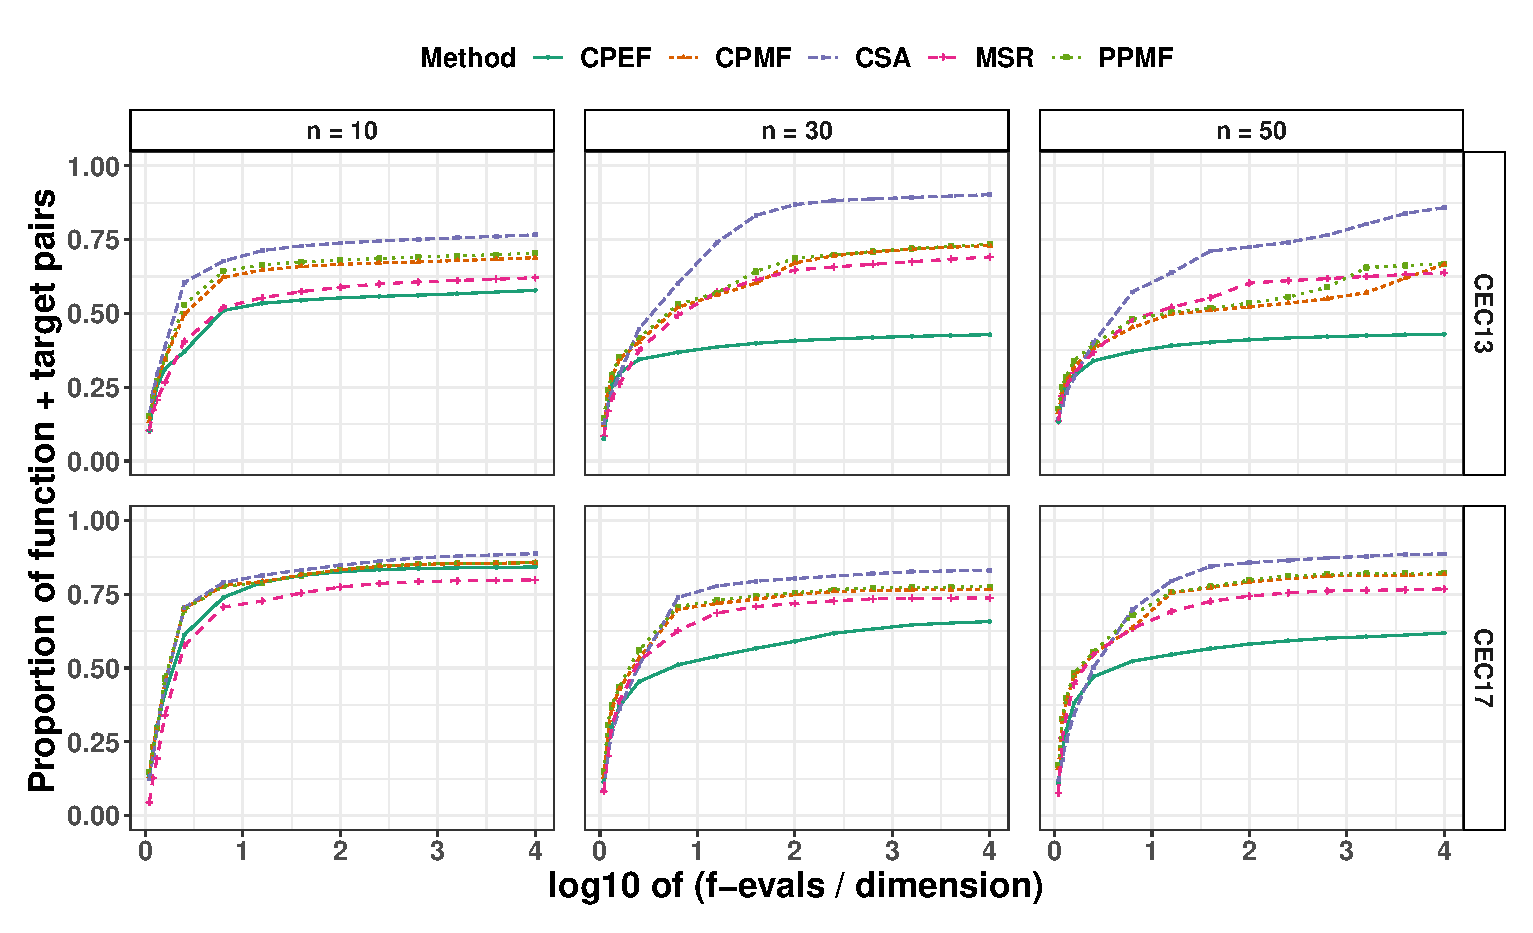
\includegraphics[width=\textwidth]{cec-17-13}
  \label{cec17-ecdf}
  \caption{ECDF curves for $D = 10, 30, 50$}
\end{figure}

\begin{figure}[H]
  \centering
  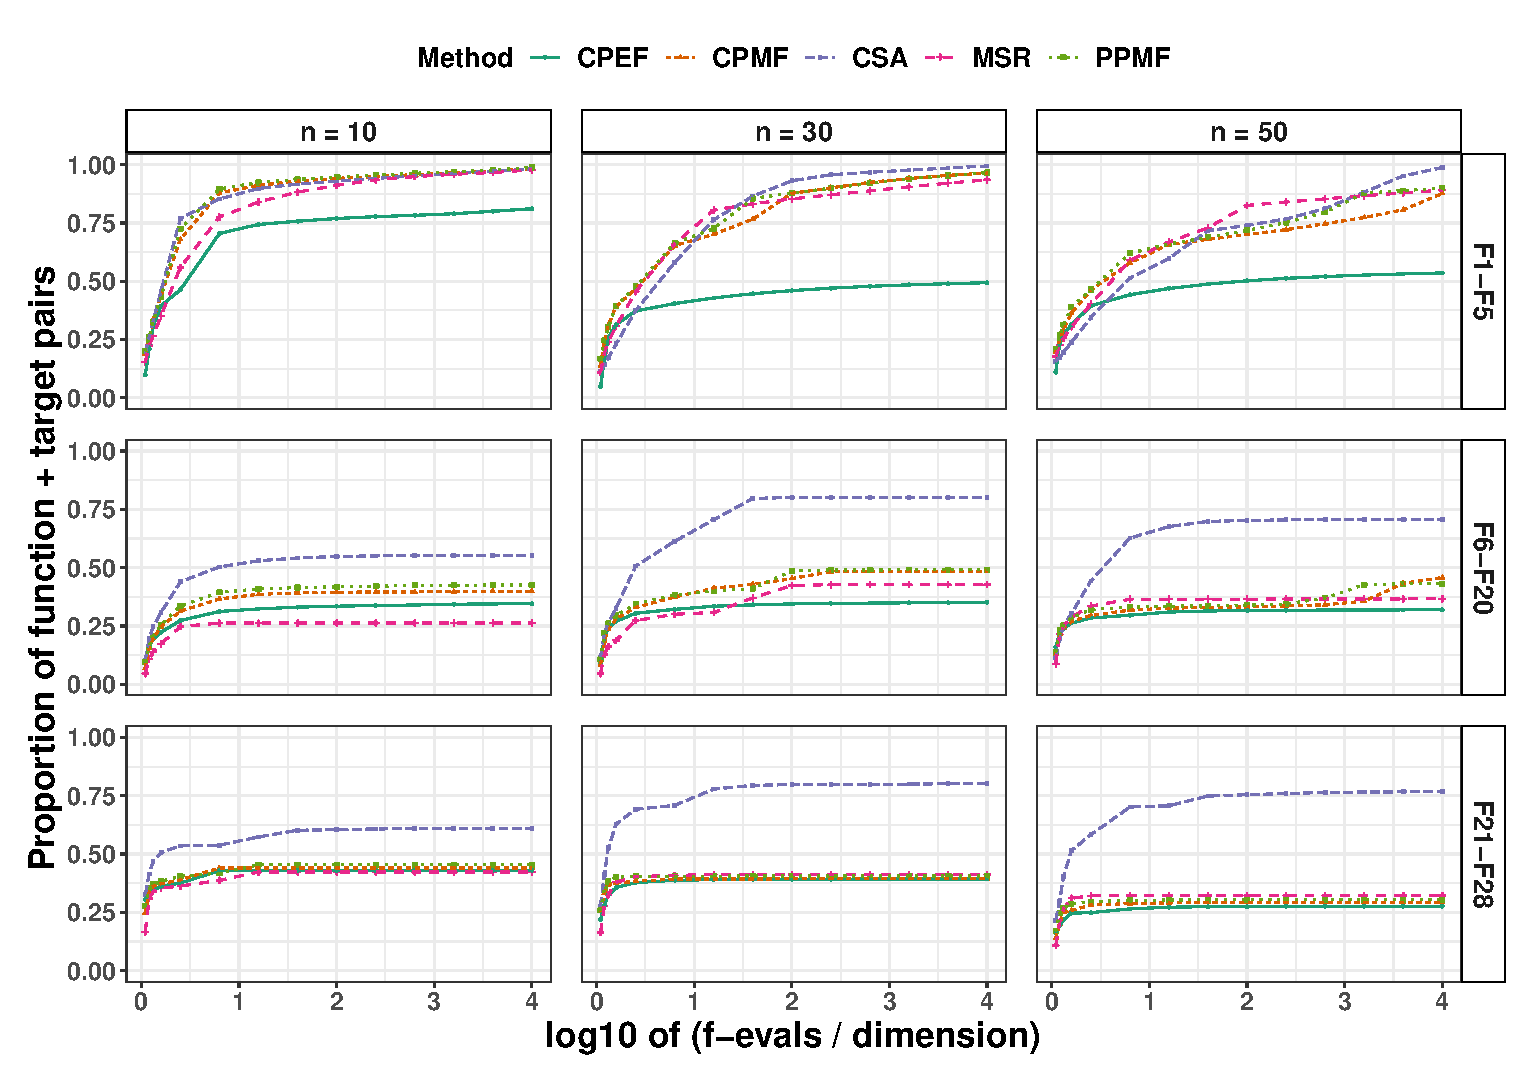
\includegraphics[width=\textwidth]{problems-cec-13}
  \label{cec17-ecdf}
  \caption{ECDF curves for $D = 10, 30, 50$}
\end{figure}


\begin{figure}[H]
  \centering
  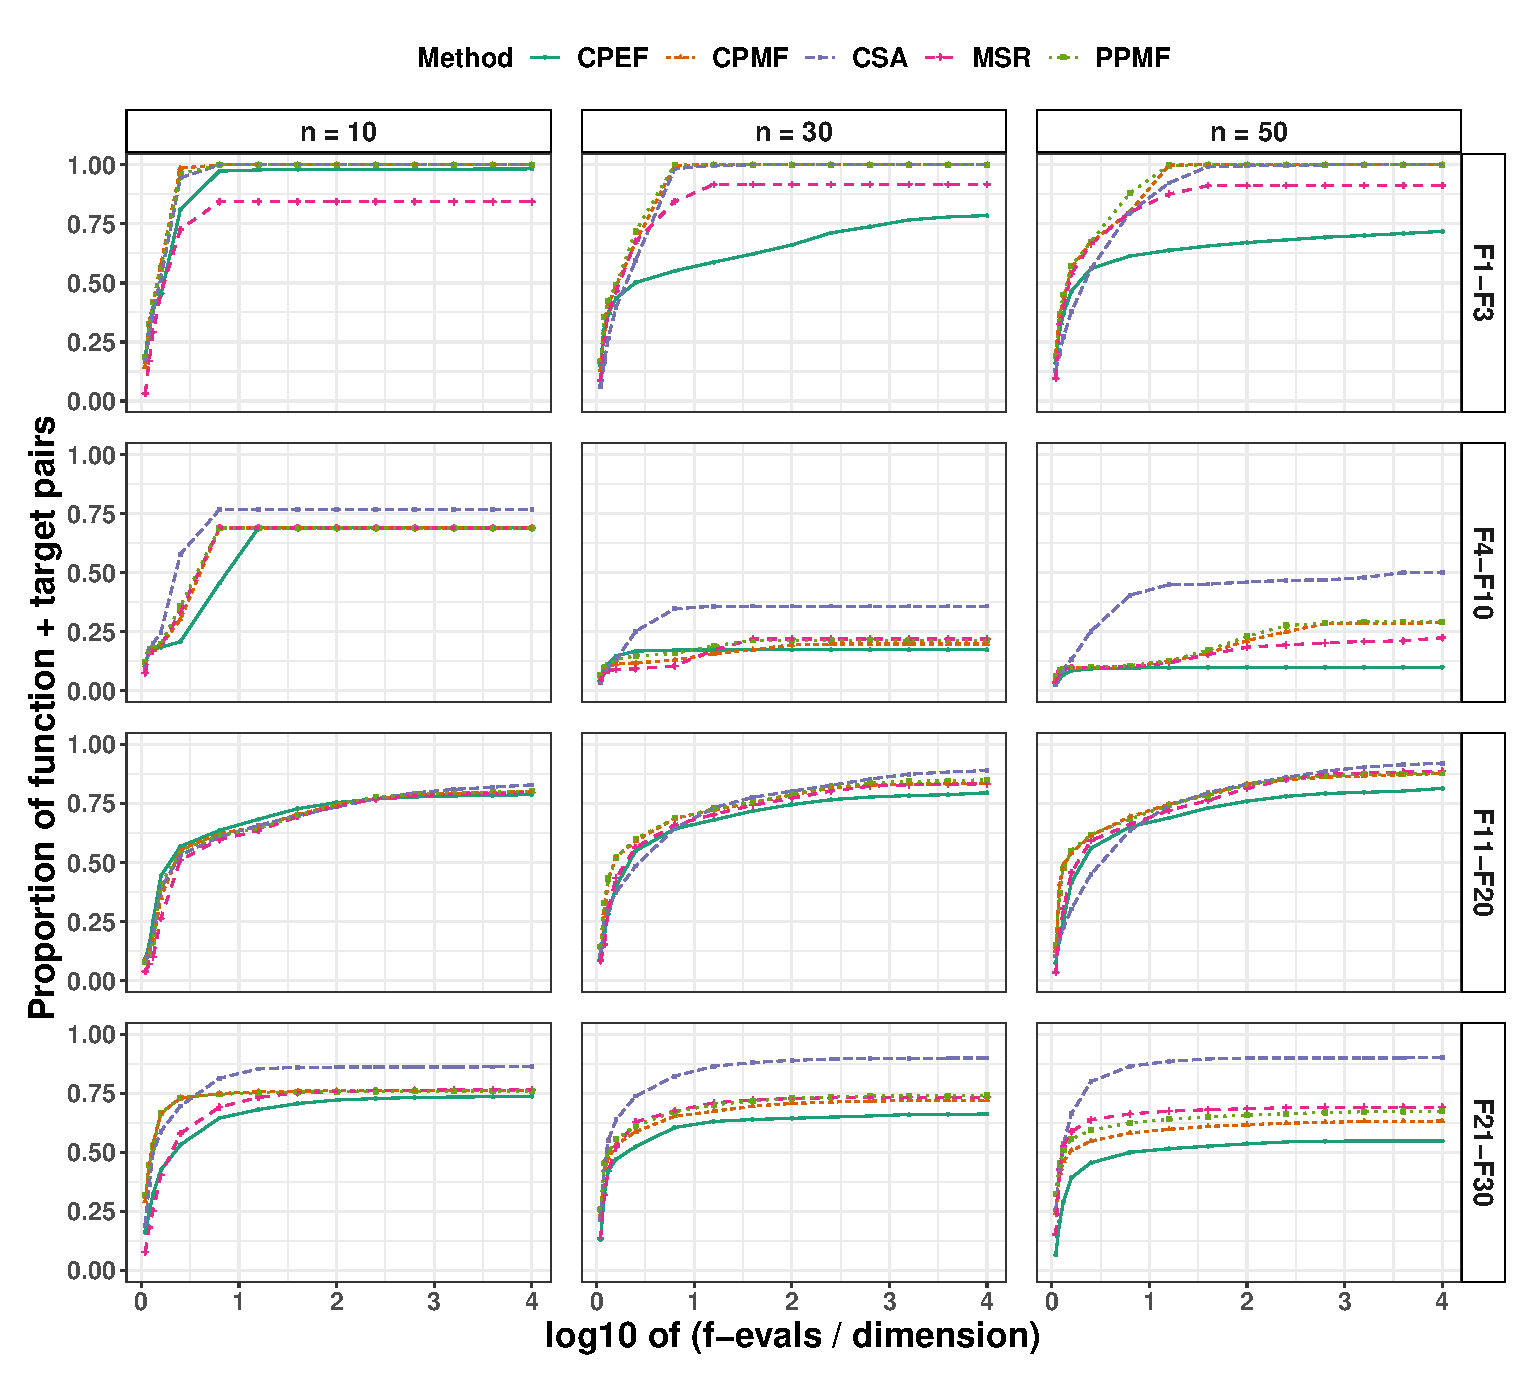
\includegraphics[width=\textwidth]{problems-cec-17}
  \label{cec17-ecdf}
  \caption{ECDF curves for $D = 10, 30, 50$}
\end{figure}


%We set the fractions as:
%\begin{equation*}
  %\{0.01, 0.02, 0.03, 0.05, 0.1, 0.2, 0.3, 0.4, 0.5, 0.6, 0.7, 0.8, 0.9, 1.0\}
%\end{equation*}

\section{Conclusions}

1. which method is advisable
{\bf  JA+EW}

2. how much computing we can spare by avoiding matrix operations
{\bf  JA+EW}

3. future research directions
{\bf  JA+EW}


\bibliographystyle{splncs}
\bibliography{ppsnJA}

\end{document}
\begin{figure}[htbp]
\centering
\psfrag{GR}[Bc][Bc][1][0]{Layer thickness (nm)}
\psfrag{LA}[Bc][Bc][1][0]{Layer \#}
\vspace{-0.5cm}
a)\includegraphics[width=3.7cm]{BRAGGGr.ps}
b)\includegraphics[width=3.7cm]{CMGr.ps}
c)\includegraphics[width=3.7cm]{DCM0Gr.ps}
\vspace{-0.3cm}
\caption{Layers thickness of: a)Bragg mirror, b)single chirped Bragg mirror, c)$\mathrm{DCM}_0$}
\label{LAY_TH}
\end{figure} 


